% !TEX root = ../../../main.tex
% 来源：中学数学实验教材·第三册（高中数学）
% 章节：函数及其图象 / 一次函数（线性函数）
% 原始文件：4.tex，行 2071-2086
% 类型：tikz
% ---
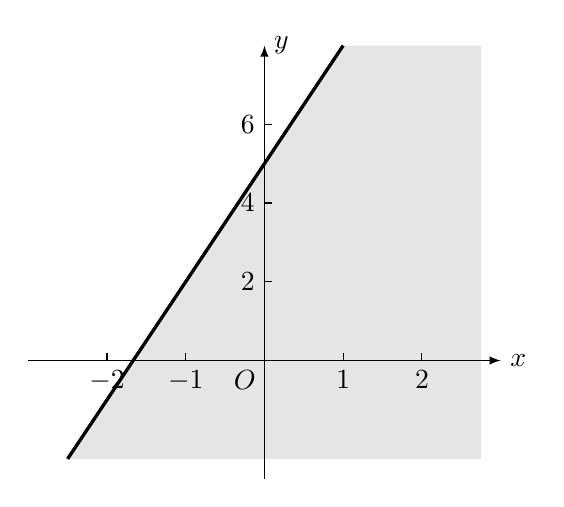
\begin{tikzpicture}[>=latex, yscale=.5]
\fill [gray!20] (-2.5,-2.5)--(1,8)--(2.75,8)--(2.75,-2.5)--(-2.5,-2.5); 
   \draw[->] (-3,0)--(3,0)node[right]{$x$};
    \draw[->] (0,-3)--(0,8)node[right]{$y$};
    \node at (-.25,-.5){$O$};   
\foreach \x in {-2,-1,1,2}
{
    \draw (\x,0)node[below]{$\x$}--(\x,.2);
}
\draw [domain=-2.5:1, samples=10, very thick] plot(\x, {3*\x+5});
\foreach \y in {2,4,6}
{
    \draw (0,\y)node[left]{$\y$}--(.1,\y);
}

\end{tikzpicture}
